\section{Interpreter Manipulation Method Examples}
\label{sec:manipulations}

After introducing the terminology of model interpreters and manipulation methods in the previous chapters, this chapter gives detailed information about recent manipulation methods. This section also provides insight into major findings in the field of manipulating model interpretations. First, input level manipulations are discussed, followed by model level manipulations. 

\subsection{Input Level Manipulations}

\mypar{Fooling both Model and Interpreter. }\newline
\cite{subramanya2019fooling} design adversarial attacks that fool the machine learning model as well as the model interpretation. 
They design targeted and untargeted input patches of various styles, which are overlaid onto the original images. 
\autoref{fig:patch_fooling} shows that GradCAM is fooled by this simple method as well as the classification model, resembling findings in research on adversarial attacks on models. 

\begin{figure}[ht]
    \centering
    \begin{subfigure}{0.32\linewidth}
      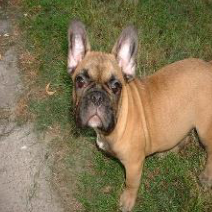
\includegraphics[width=\linewidth]{figures/patch_original.png}
      \caption{\scriptsize{Original. \newline Pred: 'French bulldog'.}}
      \label{fig:patch_original}
    \end{subfigure}
    \begin{subfigure}{0.32\linewidth}
      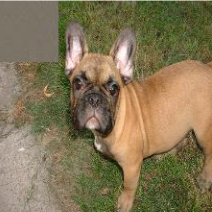
\includegraphics[width=\linewidth]{figures/patch_plus_dog.png}
      \caption{\scriptsize{Original with\newline Patch.}}
      \label{fig:patch_plus_dog}
    \end{subfigure}
    \begin{subfigure}{0.32\linewidth}
      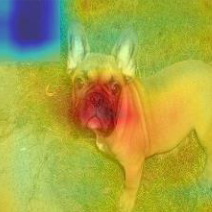
\includegraphics[width=\linewidth]{figures/patch_fooled.png}
      \caption{\scriptsize{Fooled Map, fooled \newline model. Pred: 'Soccer ball'.}}
      \label{fig:patch_fooled}
    \end{subfigure}
    \caption{Fooling of the model and GradCAM. The interpreter is deceived as it takes the features of the original target class as evidence of the wrong class. Images from \cite{subramanya2019fooling}.}\label{fig:patch_fooling}
    \vspace{-0.3cm}
\end{figure}

\mypar{Imperceptible Perturbations significantly alter interpretations. }
\cite{dombrowski2019explanations} show the pendant of adversarial model attacks for interpretation methods: They apply visually imperceptible perturbations to input images, that do not cause the model to misclassify but that cause the interpreter to yield significantly different interpretations. Perturbed images are constructed by using a generative model minimizing the distance to a target map, see \autoref{fig:dombr}. They also propose to make interpretation results better by smoothing the interpretation process, thus providing a way to undo the fooling of the interpreters (e.g. using $\beta$ smoothing).

\begin{figure}[ht]
    \centering
    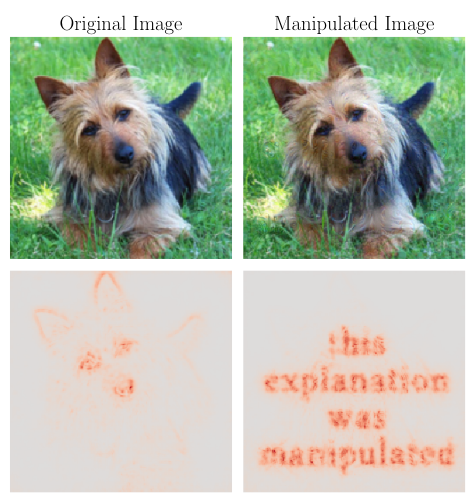
\includegraphics[width=0.8\linewidth]{figures/dombr.png}
    \caption{On the left, the original image with corresponding interpretation map is shown. The right column shows the imperceptibly perturbed input image and it's explanation. The target interpretation map was chosen to be an image with the text "this explanation was manipulated". Image from \cite{dombrowski2019explanations}.}\label{fig:dombr}
    \vspace{-0.3cm}
\end{figure}

\mypar{Saliency Maps are vulnerable to Adversarial Attacks.}
\cite{ghorbani2019interpretation} showed that importance scores produced by the popular the saliency-based interpretation methods SimpleGrad, DeepLIFT and Integrated Gradients are susceptible even to random perturbations. Contrary to \cite{dombrowski2019explanations}, the authors argue that the interpretation methods are actually not broken by these perturbations. They state that saliency-map based approaches are very sensitive, thus reacting to the infinitesimal perturbation of an input $\mathbf{x}$ to $\mathbf{x}+\delta$ with an appropriate change in their output.

\subsection{Model Level Manipulations}
The studies on model manipulation outlined so far have shown that \textit{input perturbations} can make interpretations worse for the same model and interpreter. The articles in this section show that \textit{perturbed model parameters} can also make explanations worse for the same input and interpreter.

\mypar{Adversarial Model Fine-Tuning Fools Multiple Interpreters.}\newline
\cite{fooling_nn_interpreters} were the first to introduce adversarial model manipulations for fooling interpretation methods. The authors adapted the fine-tuning stage of image classification models by using an altered fooling loss function. This loss function is a combination of the standard cross entropy loss function (to maintain the prediction performance) and an additional adversarial term. The adversarial term is used to encourage the interpretation method to give bad interpretations. The results show that the interpretation results are significantly altered while the classification accuracy is maintained. 
This indicates, that the model is robust to the attack, while the interpretation technique is very sensitive. 
Two categories of fooling methods are introduced: 
\begin{itemize}
    \item \textbf{Passive Fooling}, describing the adaption of the adversarial loss term to fool the interpretation method into highlighting uninformative pixels in the input image. They develop three types for this, namely top$-k$, center and location fooling. Example results from the paper are in \autoref{fig:heo_intro}, columns two to four. The baseline column shows that the interpretation method applied to the original image highlights pixels within the elephant as highly important for the network prediction. After fine-tuning the model with the adversarial loss, the effect of fooling the interpretation method is visible: Other, rather uninformative pixels are highlighted (see labeled columns two to four in the figure). 
    \item \textbf{Active Fooling} is a method with the aim of causing the interpreter to highlight a completely different object in the image, i.e. to make the interpreter actively create false interpretations. This is achieved by fine-tuning the model on input images that contain instances from two classes, say the $c_1$=\textit{elephant} and $c_2$=\textit{fire truck} class. The loss with a penalty term that alters the explanations of $c_1$ and $c_2$. The effect of this successful active fooling can be observed in \autoref{fig:heo_intro}, rightmost column.
\end{itemize}

\begin{figure}[ht]
    \centering
    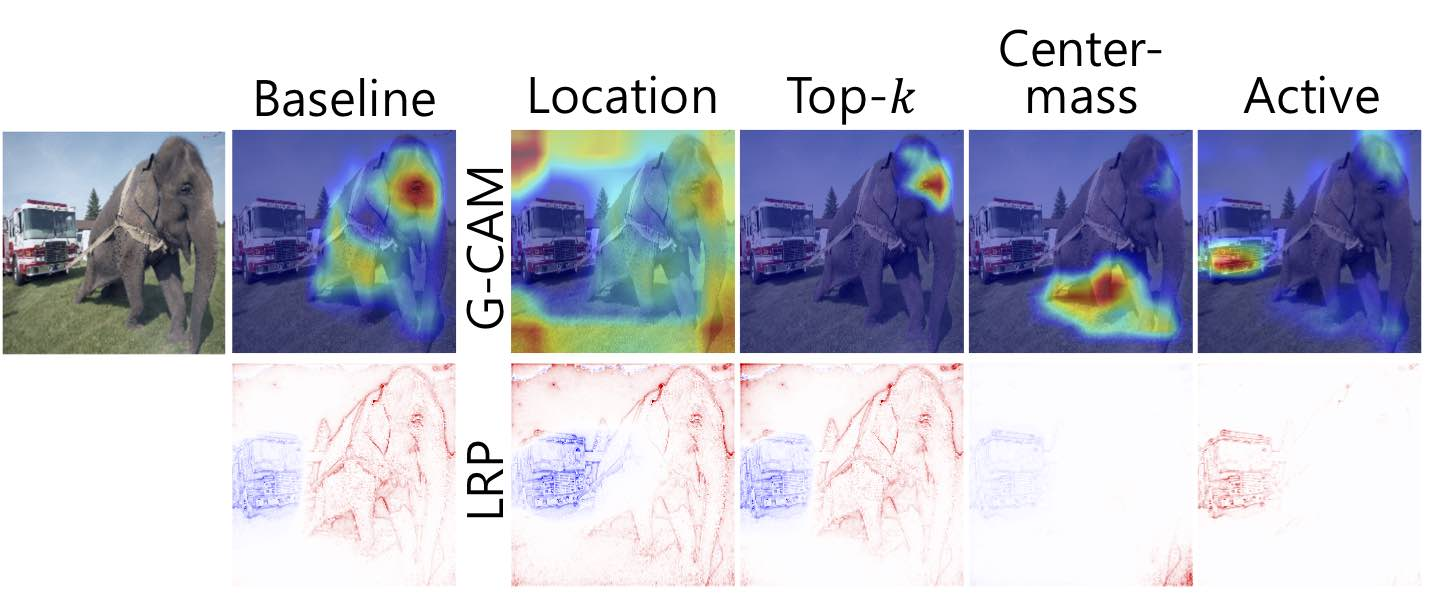
\includegraphics[width=\linewidth]{figures/heo_intro.jpg}
    \caption{Fooling of LRP and GradCAM. Passive fooling causes the interpreters to highlight wrong, uninformative pixels. Active shifts the interpreters indications from a correct (\textit{elephant}) to a wrong class \textit{(fire truck}). Image from \cite{fooling_nn_interpreters}.}
    \label{fig:heo_intro}
    \vspace{-0.3cm}
\end{figure}

% The authors also conduct quantitative analysis using the AOPC metric to prove that the interpretations found by the interpreters are valid.
 They find that all tested interpreters are fooled to a certain degree, and that the interpreter malfunctions furthermore generalize to other interpreters and especially to the whole validation set. It is worth noting that the proposed attack could not easily fool SmoothGrad, indicating that this is a better, or at least more robust interpretation method. 

The main point the authors are trying to make is that machine models can be systematically manipulated to contain unfair biases. They prove that such biases can be explicitly encoded into the loss function during the training stage, which yields an adversarial classifier that will generalizes the learned bias to unseen test samples. This is dangerous, as the bias cannot be uncovered unless one has access to the full training pipeline. 

\mypar{Model-agnostic Interpreters can be gamed and model biases can be hidden.} 
%%%%%%%%  %%%%%%%% Fooling LIME and SHAP: Adversarial Attacks on Post hoc Explanation Methods
% https://arxiv.org/pdf/1911.02508.pdf 
\cite{advlime_aies20} propose a framework for fooling the model-agnostic interpreters LIME and SHAP. 
The authors take a statistical approach to fooling model-agnostic interpretation methods. They examined the data produced by LIME's and SHAP's perturbation schemes and showed that the perturbed samples are out-of-distribution (o.o.d.) samples compared to the distribution of the regular training data. The authors used this insight, i.e. that LIME and SHAP heavily rely on o.o.d. samples and are thus o.o.d. classifiers, to train an adversarial classifier: This classifier exhibits biased behavior (e.g. using the feature 'race' for predicting the income class of a person) on instances from the original data distribution, while using insensitive features for predicting on o.o.d. samples. It is shown that the interpreters are not able to detect the model bias as they create innocuous interpretations. However, LIME performs slightly better than SHAP. 

This adversarial framework is applied to numerous real-world datasets, and are thus one of the few papers \textit{not} considering computer vision tasks but rather tasks that actually suit the core motivational concern in XAI: That models might be adversarial und unbiased, and that we might not be able to detect that their decision functions are unfair, racist or discriminatory. 

\mypar{Learning Models Which Conceal Unfairness.}
\cite{dimanov2020you} examine the relation of interpretation methods and the concept of fairness. They propose to learn a modified model with concealed unfairness. Their approach differs methodologically to \cite{fooling_nn_interpreters} as follows: 
\cite{fooling_nn_interpreters} adapt the standard cross entropy loss function by taking the gradient of the correct label element from the logits layer, while \cite{dimanov2020you} use the gradient of the cross-entropy loss instead. 
Taking the gradient of the cross-entropy loss conveys more information about other classes, which may contribute to an improved generalization across different interpretation methods and first of all across different test samples. 
Using this method, they are also able to create adversarial models that focus only on sensitive features which are not informative for the ground truth decision. Again, this hidden bias cannot be detected by the examined interpreters. 
